\documentclass[../../main/main.tex]{subfiles}

\begin{document}

\section{Methods}
\label{sec:methods}


\subsection{ The Model architecture}
\label{sec:model-architecture}

The architecture of the neural network consist of two hidden layers that each has 1000 nodes and where we use the RelU activation function. The input layer has a varying number of nodes depending on how the higgs dataset is used which will be described in Section ... The output of the neural network is given from one node where we use the Sigmoid activation function to keep the output between 0 and 1. We use the binary cross entropy loss function which also will be used to estimate the log likely ratio function. The L2 reguralization is used.
\subsection{The Higgs dataset and collision physics}
\label{sec:higgs-dataset}

The dataset used for the HiggsML challenge consist of the output of simulated collisions, called \emph{events}, and is provided by the ATLAS experiment at CERN. The HiggsML dataset consist of 35 features which are given in Table ... (remember to put in Weight, count) in which of them contains the information about the kinematics of the outgoing particles in the events. We do not include the features \texttt{EventId}, \texttt{Weiht}, \texttt{KaggleSet} and \texttt{KaggleWeight} in the training of the neural network since they are not relevant for the physics of the collisions. In order to understand how we can use the dataset in the neural network, and the challenges that it gives we will give a brief introduction to the physics of the collisions in the ATLAS detector that has been used to simulate the events for the dataset.

The ATLAS detector is one of the detectors at the Large Hadron Collider (LHC) where two opposing proton beams collide and the outgoing particles from the collision is measured by the detector and is called the final state particles. Figure \ref{fig:ATLAS} shows the referance frame of the sylindrical ATLAS detector where the two proton beams going in opposite direction along the \(z\)-axis collide in the origin of the coordinate system.

\begin{figure}[H]
  \centering
  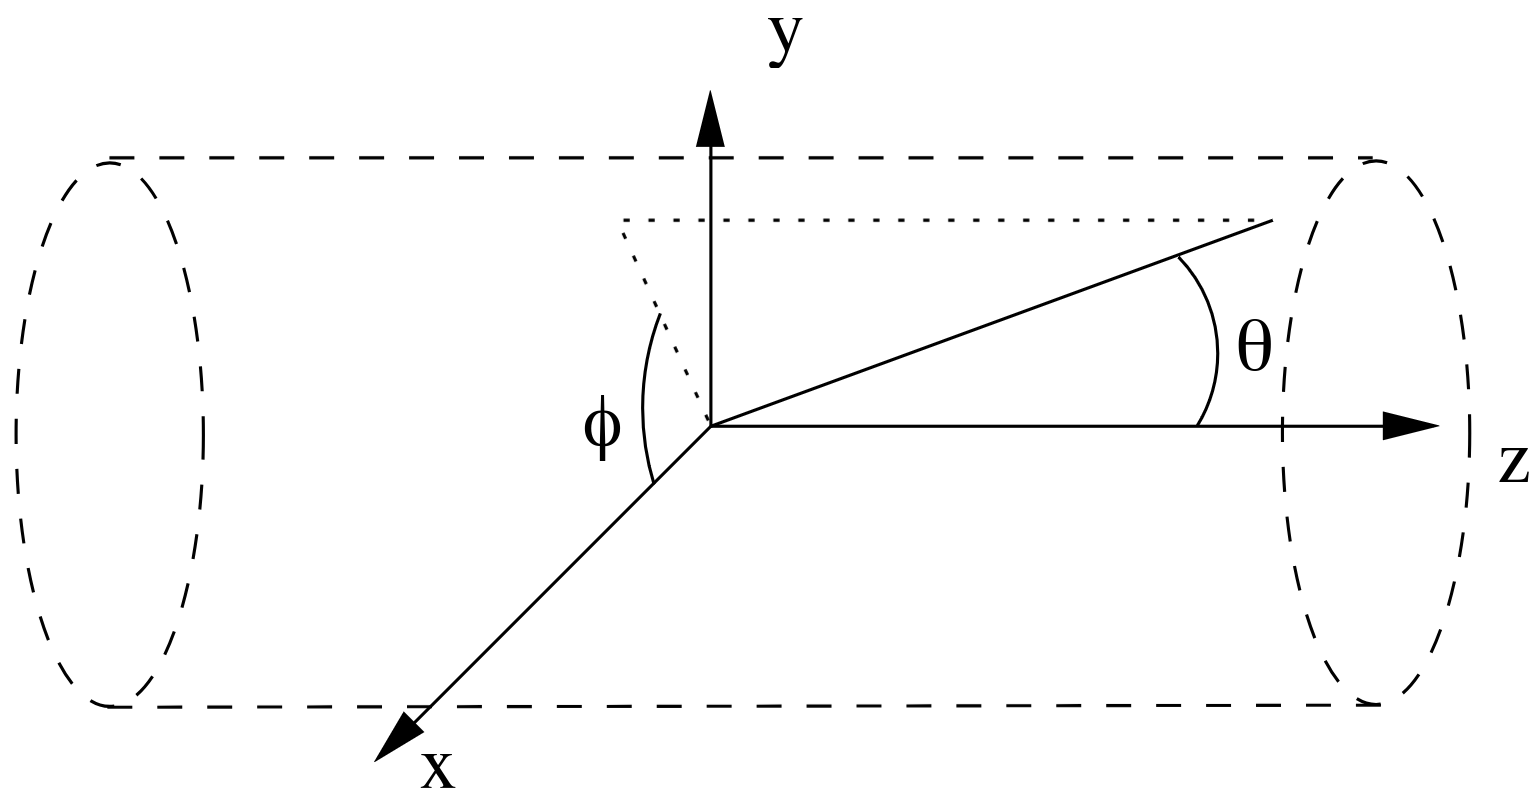
\includegraphics[width = 0.8\linewidth]{../../figures/ATLAS-reference-frame.png}
  \caption{ALTAS reference frame}
  \label{fig:ATLAS}
\end{figure}

The azimuthal angle \(\phi\) is used to measuasre the direction of the particles in the \(x\)-\(y\) plane while the polar andlge \(\theta\) is used to meusure the direction of the particle from the \(z\)-axis. In particle physics we often use what is called the \emph{psuedorapididy} \(\eta\) instead of \(\theta\), and is given as \(\eta=-\ln(\tan(\theta/2))\). The momentum of a particle meausured in the \(x\)-\(y\) plane is called the \emph{transverse momentum} and is denoted \(p_T\). The final state particle present in the events used for the HiggsML dataset is a tau tau pair that could come from the decay of e.g a \(Z\) boson or the Higgs boson. We call an event where the tau tau final state has decayed from a Higgs boson a \emph{signal event} and an event where the two tau's comes from the decay of other particles like the \(Z\) boson a \emph{background event}.

The goal of the Higgs challange is to be able to distingusihe the signal and background events from each other in order to discover the Higgs boson, and it is therefore a binary classification problem. In the HiggsML dataset the signal and background events are denoted by \(s\) and \(b\) respectively in the feature named \texttt{Label}, and we replace \(s\) and \(b\) by 1 and 0 respectively such that the dataset can be used in the neural network. This is also why we use one output node to classify the event.

In addition to the tau particle there may also be jets present in the event that comes from the hadronisation of quarks. The features include the kinematics from the particles like the transverse momentum of the taus and jets in addition to the angles \(\phi\) and \(\eta\) from Figure ... . Not all events have jets, so for these events the features assisated to the leading and subleading jet does not have any values. Table ... shows the features in the dataset marked with a checkmark if they have a value for the different events with 0, 1 or 2-3 jets. We call the variables that does not have a value for every event a \emph{missing variable} and becomes a challange for the neural network since it requires that every feature has a value. We describe how to deal with the missing variabels in the data set in Section . In addition some events also has what is called \emph{jets} that is produced from the hadronization of the quarks in the detector. It is common to order the jets after their transverse momentum \(p_T\), and we call the jet with the highest \(p_T\) the \emph{leading jet} and the jet with the next to highest \(p_T\) the \emph{subleading jet}. When it comes to the HiggsML dataset we will study closer how we can deal with the events in the dataset that has either no subleading jet, or both no subleading and leading jet. In the HiggsML datasets the number of jets is described by the feauture \texttt{PRI\_num\_jet} and takes the values 0, 1, 2 and 3.

\begin{table}[H]
  \centering
  \caption{Fraction of jets}  
  \begin{ruledtabular}
    \begin{tabular}{l|lll}
      \(n_{jets}\) & Events & Background [frac.] & Signal [frac.] \\
      \hline
      0,1,2 and 3 & 818238  & 0.658 & 0.342 \\
      \hline
      0 &  327371 & 0.747 & 0.253 \\
      1 & 252882 & 0.643 & 0.357 \\
      2 and 3 & 237985 & 0.552 & 0.448 \\
    \end{tabular}
  \end{ruledtabular}
  \label{tab:events}
\end{table}

We observe that the fraction of signal and background events is not balanced with the execption of the events with 2 and 3 jets where they are more balanced.

..
\subsection{Construction of Datasets and Missing variables}
\label{sec:missing-variables}

To deal with the missing variable in the dataset we will use three different methods that can be summarized as;
\begin{enumerate}[label=\Roman*.]
\item Inserting values into the entries with missing values
\item Remove the features that has missing variables
\item Split the data set into multiple disjoint data sets according to the number of jets, and then remove the features with missing values in the disjoint data sets
\end{enumerate}

\subsubsection*{Inserting values}
\label{sec:inserting-values}

We can use several methods to insert values into the entries that has missing values in the data set. Two of the methods that we use here is to either insert the mean value from each jet variable in the missing entries or insert zero in all the missing entries. We will reffer to these methods as \emph{fillMean} and \emph{fillZero} respectively. For the third method that we use is to use the observation that the \(\phi\) variables is almost uniformly distributed between \(-\pi\) and \(\pi\) as shown in Figure ... From this observation we use to insert a random variable between \(-\pi\) and \(\pi\) for the missing entries in the \(\phi\) variables and then insert the mean value in the other jets variables. We refer to this method as \emph{fillPhiRandom}. In all these datasets none of the feautures are removed so there are 30 feautures in each of these datasets.

\subsubsection*{Removing features}

Another way of dealing with the missing variables is to remove the features that has missing values in them. These feautures include the jet variables and the DERmass variable. In the first method with removing feautures we remove all the jet feautures to get rid of the missing variables in the data set. Because the DERmass variable only has 15\% missing variables and is not directly conneted to the jets we do not remove it, but insert the mean value instead. We refer to this method as \emph{removeJets}. The number of feautures in this dataset is reduced from the to 20 feautures from the original Higgs dataset. In the second model we also in addition remove all the \(\phi\) features since they have an almost uniform distrubution, and therefore a large variance. By doing this we get a measure on how important \(\phi\) features are for the prediction of the background and signal events, and we refer to this method as \emph{removePhi}. The number of feautures in this dataset is therefore reduced to 25 feautures compared to the original dataset.

\subsubsection{Disjont datasets}
\label{sec:disjont-datasets}

The third way that we will use to deal with the missing variables is to split the data sets into three disjiont data sets according to the number of jets in the events, and then remove the feautures that has missing variables in the three cases respectively. The dataset is split into the events with 0, 1 and 2-3 jets respectively. In the case with 2-3 jets, none of the features are removed, while for 1 the features related to the subleading jet are removed, and for 0 jets both the features related to the leading and subleading jets are removed. In the datasets with 0 and 1 jets we also get some redundant features that either is unnecessary or that two feautures contain the same information. This is the case for the features PRI\_jet\_num and PRI\_jet\_all\_pt for both the events with 0 and 1 jets. The feauture PRI\_jet\_num counts the number of jets in the event and is therefore unnecessary since it contains 0 or 1 for the events with 0 and 1 jets respectively. The feauture PRI\_jet\_all\_pt gives us the sum of the \(p_T\) of all the jets in the event. In events with 0 jets the feature PRI\_jet\_num contains only 0 values since there are not jets in those events, and are therefore unnecessary. For the events with 1 jet the feature PRI\_jet\_all\_pt gives the same value as the \(p_T\) of the leading jet in the event given in the feauture PRI\_jet\_leading\_pt, and the information in PRI\_jet\_all\_pt is therefore redundant. We will refer to the datasets with 0, 1 and 2-3 jets as \emph{JetsNone}, \emph{JetsOne} and \emph{JetsTwo} respectively, and contains 18, 21 and 30 feautures respectively.

  


\begin{table}[H]
  \centering
  \begin{ruledtabular}
    \begin{tabular}{l|lll}
      \(n_{jets}\) & Events & Background [frac.] & Signal [frac.] \\
      \hline
      0,1,2 and 3 & 818238  & 0.658 & 0.342 \\
      0 &  327371 & 0.747 & 0.253 \\
      1 & 252882 & 0.643 & 0.357 \\
      2 and 3 & 237985 & 0.552 & 0.448 \\
    \end{tabular}
  \end{ruledtabular}
  \caption{Fraction of jets}
  \label{tab:events}
\end{table}



\end{document}